\documentclass[a4paper,%foobar
twoside]{article}

\newcommand{\uuid}[1]{}%{{\texttt[#1]}}

\usepackage{mypackage}

\def\nr{4}
\def\nr_b{3}

\newcommand{\NR}{5}
%\newcommand{\NR_B}{6}

\usepackage[english]{babel}

\usepackage[margin=18ex %,headheight=16pt
]{geometry}

\usepackage{amsthm,amsmath}

\usepackage{graphicx}

\newcounter{myCount}

\newtheorem{Theorem}%
[myCount]{Teorema}

\newtheorem*{Cor}%comment
{Corollary}

\newtheorem{Lem}%comment [myCount]
{Lemma}

\newcommand\prerequisites[1]{{[Pre:#1]}}
\begin{document}
\section{test input}
%
Hellodear,how

are you?

Double input my dear!

\section{first}%comment
the number \nr_b

A citation \cite{wiki:it:tautol}

\begin{Theorem}[A  Theorem for {$I=]0,1[$}]
  % A comment after the option
  \label{CT}
  The formula
\[ \int_I {\sin(c)} \hbox{is an \textbf{integral}}\]
\end{Theorem}

A short paragraph of text; this should not be in a separate blob.

\begin{Cor}
  % a comment , no option
  \label{CC}
  The other formula
  \begin{equation}%
    \label{eq:CC}
    \int_{\cos(c)} < \e
  \end{equation}
\end{Cor}
\begin{Lem}\label{lem:2}
  \prerequisites {\emph{that chap}}
  Then a Lemma citing the equation \ref{eq:CC} of the un-numbered Corollary \ref{CC}
\end{Lem}

\begin{Theorem}% a comment before the option
  [Another Theorem]
  % a comment after the option but before the label
  \label{AT}
  The formula
  \[ \int_I{e^{f^{g(x)}}} \ \textbf{d}x \]
  and a citation to the first Theorem \ref{CT}
\end{Theorem}

%\begin{Cor}[A Corollary with a LaTeX mistake]\label{CM}
%  There is a deliberate LaTeX mistake here: \foobarbaz
%\end{Cor}

\section*{second $\int$}

\begin{center}
  include with extension PDF
  \\
  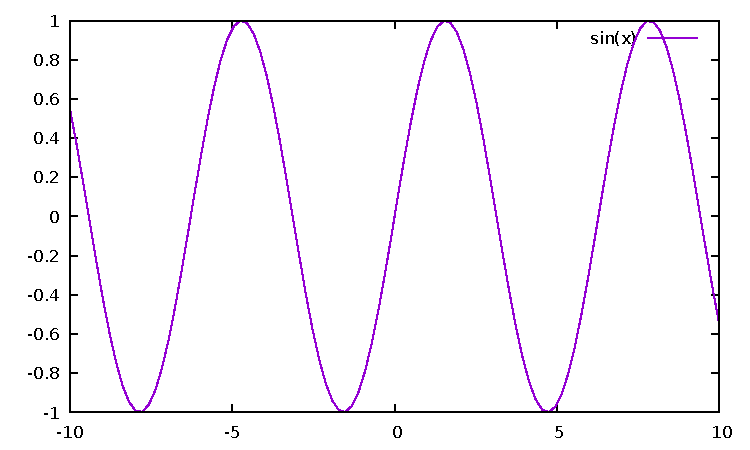
\includegraphics[width=0.5\textwidth]{F/sin.pdf}
  \\
  include with extension PNG
  \\
  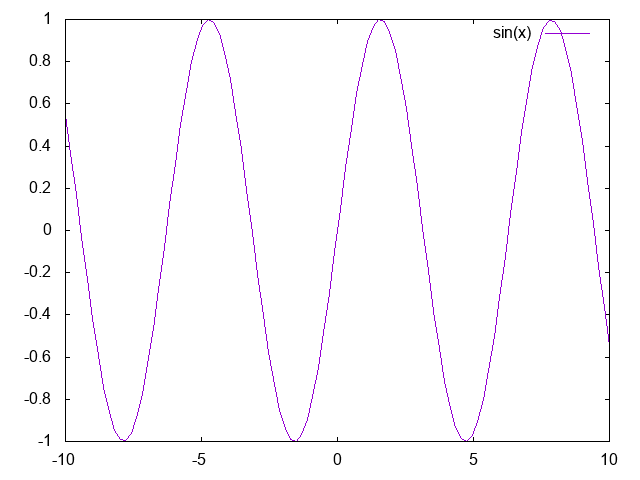
\includegraphics[width=0.5\textwidth]{F/sin.png}
  \\
  include smaller
  \\
  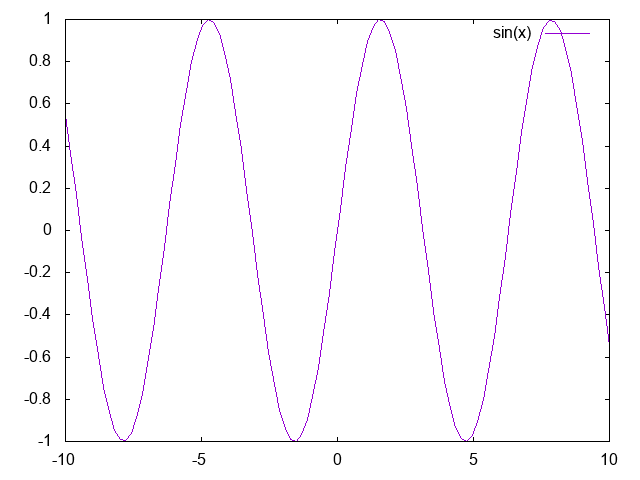
\includegraphics[width=0.2\textwidth]{F/sin.png}
  \\
  include without extension
  \\
  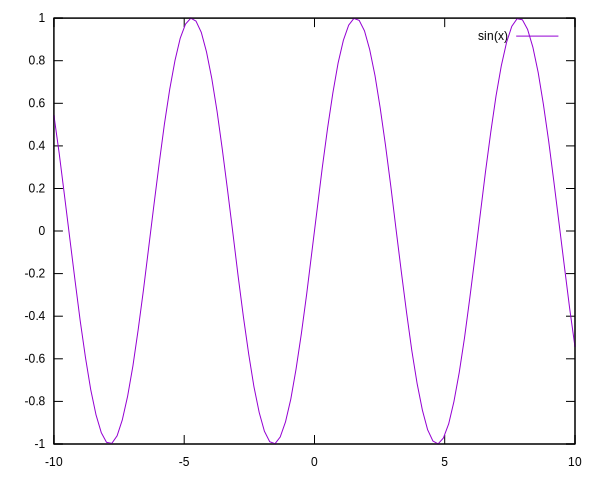
\includegraphics[width=0.5\textwidth]{F/sin}
\end{center}


a complex command
\emph{ital\`ic\textsl{~\~slanted\_\texttt{writer\_%
      \_macro}}}
\textbf{only boldface}

\begin{itemize}%comment

%comment

\item one
\item two
\end{itemize}


\begin{verbatim}
a verbatim
 \int_\label{343}
 \begin{Theorem}
\section*{A list inside an equation}%comment
yes you can
\begin{equation}
 \int \sin \quad \text{\fbox{\parbox{0.4\textwidth}{ is a simple integral that computes to   }}} =\cos
\end{equation}


\begin{equation}
 \int \sin \quad \text{\fbox{\parbox{0.4\textwidth}{        \begin{itemize}
       \item is a simple integral
       \item it can be shown to be equal to
       \end{itemize}
  }}} =\cos
\end{equation}



%%% Local Variables:
%%% mode: latex
%%% TeX-master: "latex_test1"
%%% End:

\input{UUID/pippo/pollo}
\end{verbatim}

\verb=a verbatim $\int$ and \input{UUID/nonexistent} =

%
\section*{A list inside an equation}%comment
yes you can
\begin{equation}
 \int \sin \quad \text{\fbox{\parbox{0.4\textwidth}{ is a simple integral that computes to   }}} =\cos
\end{equation}


\begin{equation}
 \int \sin \quad \text{\fbox{\parbox{0.4\textwidth}{        \begin{itemize}
       \item is a simple integral
       \item it can be shown to be equal to
       \end{itemize}
  }}} =\cos
\end{equation}



%%% Local Variables:
%%% mode: latex
%%% TeX-master: "latex_test1"
%%% End:

%

\section{third $\cos$}

This section may be ``zipped'' if
the option \verb+--ZS+ is given
\verb+blob_inator+

``Not zipped'' means that there will be a blob X
generated by \verb+\section{third $\cos$}

This section may be ``zipped'' if
the option \verb+--ZS+ is given
\verb+blob_inator+

``Not zipped'' means that there will be a blob X
generated by \verb+\section{third $\cos$}

This section may be ``zipped'' if
the option \verb+--ZS+ is given
\verb+blob_inator+

``Not zipped'' means that there will be a blob X
generated by \verb+\include{sec3}+ in the main file;
and then another blob Y for this section;
the blob X will simply contain \verb+\input{Y}+

``Zipped'' means that there will be only one blob.



A long paragraph of text in section 3; this should be in a separate blob.  Sed
luctus, nisl a hendrerit tincidunt, felis mauris aliquam magna, vitae
vestibulum nibh risus vel tortor. Sed libero. Class aptent taciti
sociosqu ad litora torquent per conubia nostra, per inceptos
hymenaeos. Phasellus consequat leo id nibh. Praesent vel arcu. In
elementum dictum massa. Proin in elit sed est feugiat mattis. Donec at
turpis eu mauris rhoncus lobortis. Praesent orci dolor, malesuada vel,
ullamcorper eget, sollicitudin sed, mi. Duis lorem quam, sagittis
vitae, lobortis nec, molestie in, sem. Phasellus vel pede eget tortor
pulvinar vestibulum. Ut enim. Proin sed purus. In cursus congue
diam. Maecenas nec est non augue iaculis semper. Proin aliquet. Nulla
et ligula ut magna elementum viverra. Suspendisse sodales.
+ in the main file;
and then another blob Y for this section;
the blob X will simply contain \verb+\input{Y}+

``Zipped'' means that there will be only one blob.



A long paragraph of text in section 3; this should be in a separate blob.  Sed
luctus, nisl a hendrerit tincidunt, felis mauris aliquam magna, vitae
vestibulum nibh risus vel tortor. Sed libero. Class aptent taciti
sociosqu ad litora torquent per conubia nostra, per inceptos
hymenaeos. Phasellus consequat leo id nibh. Praesent vel arcu. In
elementum dictum massa. Proin in elit sed est feugiat mattis. Donec at
turpis eu mauris rhoncus lobortis. Praesent orci dolor, malesuada vel,
ullamcorper eget, sollicitudin sed, mi. Duis lorem quam, sagittis
vitae, lobortis nec, molestie in, sem. Phasellus vel pede eget tortor
pulvinar vestibulum. Ut enim. Proin sed purus. In cursus congue
diam. Maecenas nec est non augue iaculis semper. Proin aliquet. Nulla
et ligula ut magna elementum viverra. Suspendisse sodales.
+ in the main file;
and then another blob Y for this section;
the blob X will simply contain \verb+\input{Y}+

``Zipped'' means that there will be only one blob.



A long paragraph of text in section 3; this should be in a separate blob.  Sed
luctus, nisl a hendrerit tincidunt, felis mauris aliquam magna, vitae
vestibulum nibh risus vel tortor. Sed libero. Class aptent taciti
sociosqu ad litora torquent per conubia nostra, per inceptos
hymenaeos. Phasellus consequat leo id nibh. Praesent vel arcu. In
elementum dictum massa. Proin in elit sed est feugiat mattis. Donec at
turpis eu mauris rhoncus lobortis. Praesent orci dolor, malesuada vel,
ullamcorper eget, sollicitudin sed, mi. Duis lorem quam, sagittis
vitae, lobortis nec, molestie in, sem. Phasellus vel pede eget tortor
pulvinar vestibulum. Ut enim. Proin sed purus. In cursus congue
diam. Maecenas nec est non augue iaculis semper. Proin aliquet. Nulla
et ligula ut magna elementum viverra. Suspendisse sodales.


A long paragraph of text; this should be in a separate blob.  Sed
luctus, nisl a hendrerit tincidunt, felis mauris aliquam magna, vitae
vestibulum nibh risus vel tortor. Sed libero. Class aptent taciti
sociosqu ad litora torquent per conubia nostra, per inceptos
hymenaeos. Phasellus consequat leo id nibh. Praesent vel arcu. In
elementum dictum massa. Proin in elit sed est feugiat mattis. Donec at
turpis eu mauris rhoncus lobortis. Praesent orci dolor, malesuada vel,
ullamcorper eget, sollicitudin sed, mi. Duis lorem quam, sagittis
vitae, lobortis nec, molestie in, sem. Phasellus vel pede eget tortor
pulvinar vestibulum. Ut enim. Proin sed purus. In cursus congue
diam. Maecenas nec est non augue iaculis semper. Proin aliquet. Nulla
et ligula ut magna elementum viverra. Suspendisse sodales.



\section*{TOC}

\tableofcontents

\bibliographystyle{plain}
\bibliography{biblio}

\end{document}
